


\subsection{Probabilités}



\subsubsection{Axiomes de la théorie des probabilités}

\begin{equation*}
\left\{
\begin{aligned}
	P(A) & \geq 0\\
    P(E) & = 1\\
    A \cap B &= \emptyset \Rightarrow P(A \cup B) = P(A)+P(B)
\end{aligned}
\right.
\end{equation*}




\subsubsection{Probabilité conditionnelle et indépendance}



Probabilité conditionnelle de $A$ sous la condition $B$ ("sachant $B$") :
$$P(A|B)=\frac{P(A \cap B)}{P(B)}$$
Si A est indépendant de $B$ :
$$P(A|B)=P(A)$$
alors
$$P(A \cap B)=P(A)P(B)$$





\subsubsection{Formule de Bayes}
Cette formule est utilisée dans le cas où un évènement $B$ peut survenir à cause d'évènement $A_i$ incompatibles. Par exemple : une pièce défectueuse fabriquée par plusieurs machines différentes.
\begin{center}
	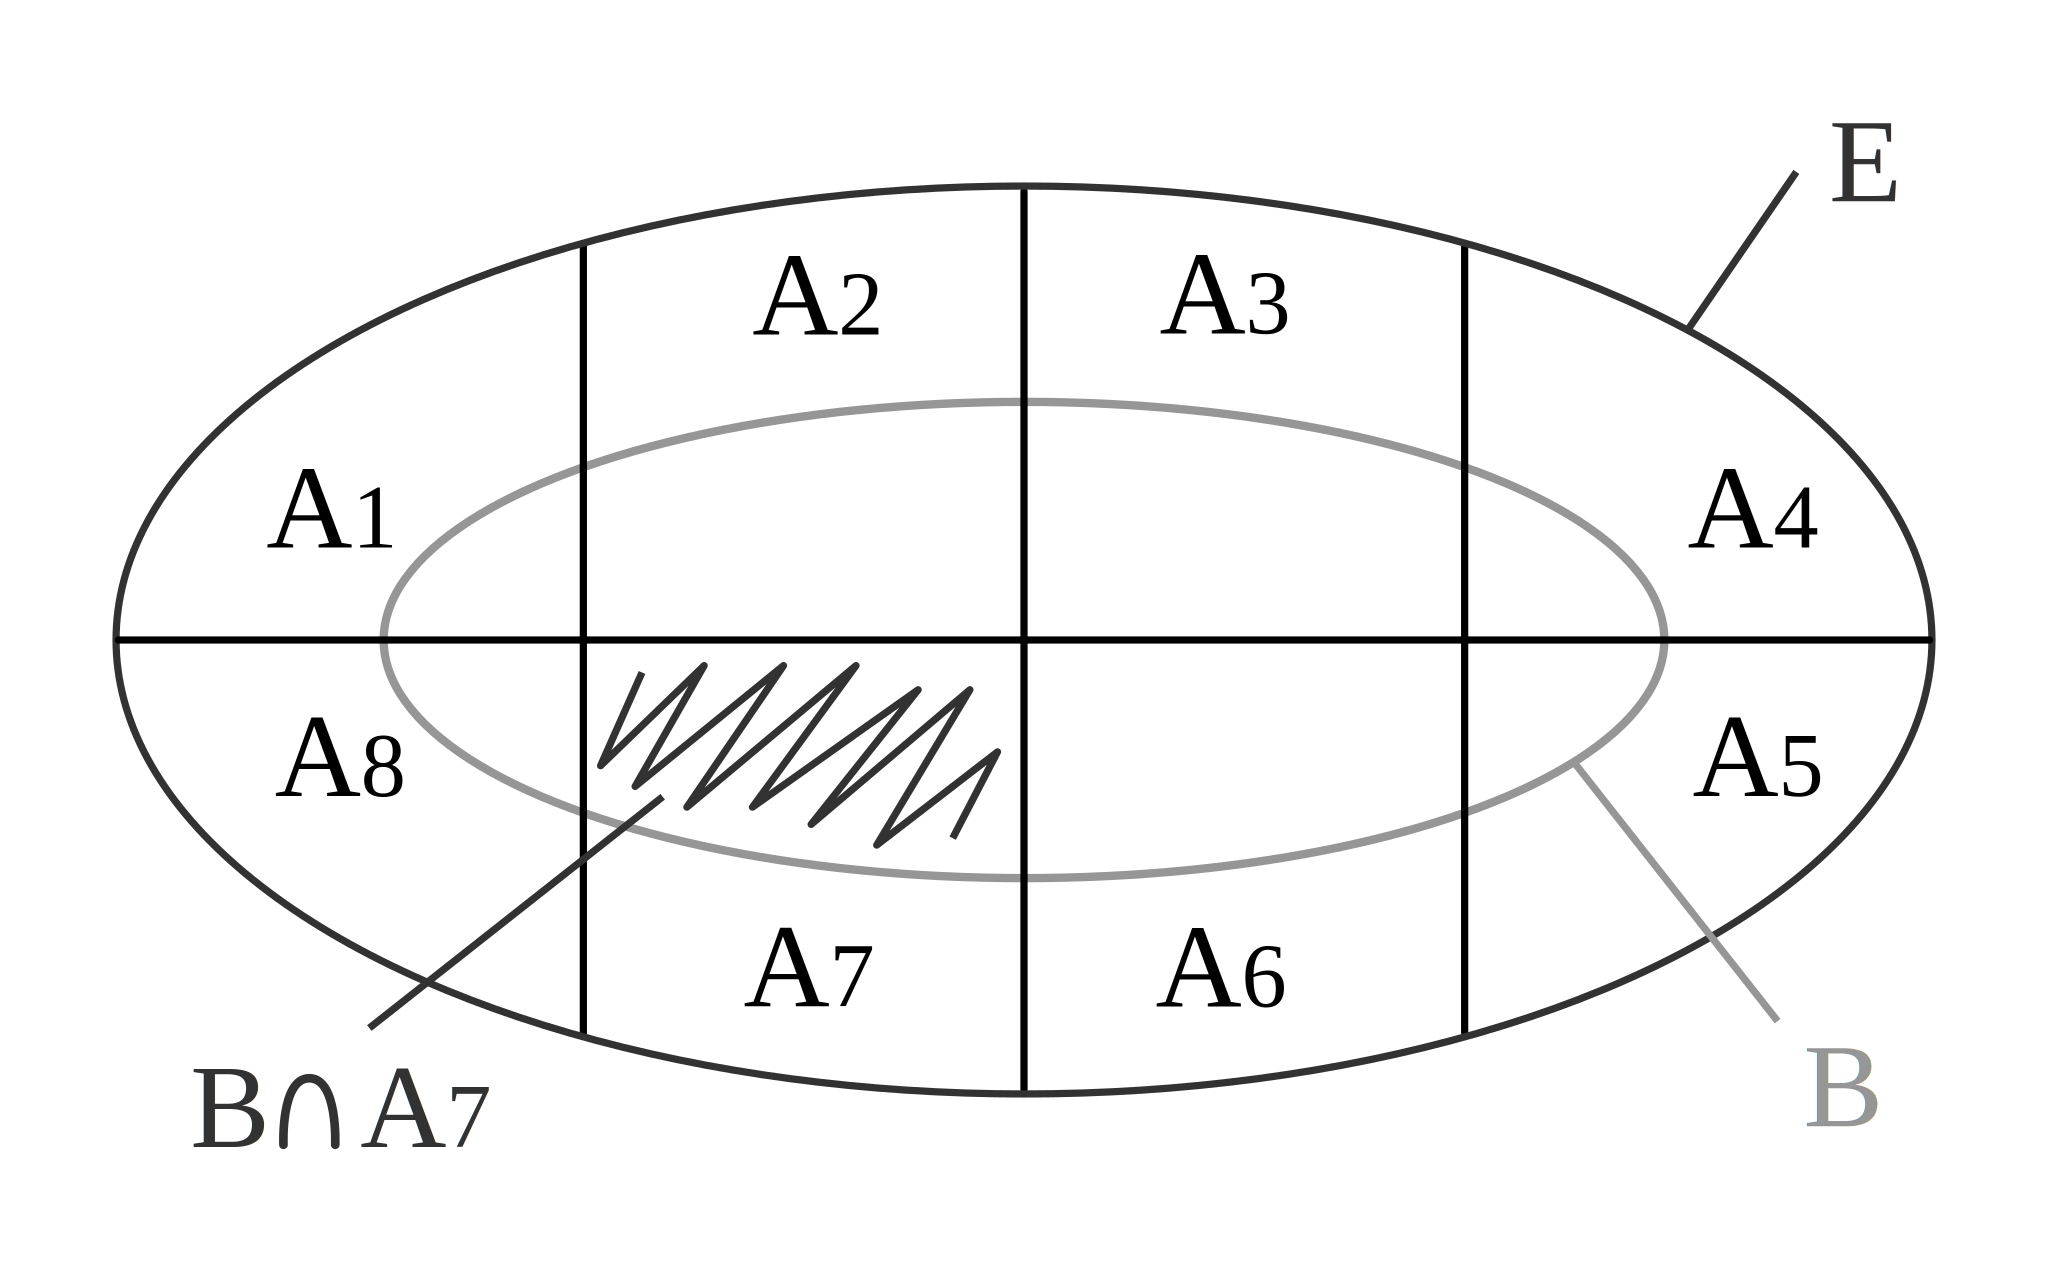
\includegraphics[width=0.3\textwidth]{images/formule-de-bayes} 
\end{center}
\begin{center}
	$\begin{array}{CCCCCCCCC}
		B    & = & (A_1 \cap B)      & \cup & (A_2 \cap B)      & \cup & \dots & \cup & (A_m \cap B)\\
		P(B) & = & P(A_1 \cap B)     & +    & P(A_2 \cap B)     & +    & \dots & +    & P(A_m \cap B)\\
		     & = & P(B | A_1) P(A_1) & +    & P(B |A_2) P(A_2) & +    & \dots & +    & P(B |A_m) P(A_m)
	\end{array}$
\end{center}

$$\boxed{P(A_k|B)=\frac{A_k \cap B}{P(B)}=\frac{P(B|A_k)P(A_k)}{\displaystyle\sum_{j=1}^{m}P(B|A_j)P(A_j)}}$$